\documentclass[a4paper, 12pt]{article}
\usepackage[T1]{fontenc}
\usepackage[utf8]{inputenc}
\usepackage{lmodern}
\usepackage[english]{babel}
\usepackage{amsmath}
\usepackage{amsfonts}
\usepackage{amssymb}
\usepackage{relsize}
%\usepackage{abraces,mathtools}
%\usepackage[hidelinks,hyperfootnotes=false]{hyperref}
\usepackage{empheq}
\usepackage{graphicx}
\usepackage{parskip}
\usepackage{indentfirst}
\usepackage[font={small, it}]{caption}
\usepackage[coverpage]{polytechnique}

\title{Specificity and constraints in Peptide-Protein bindings in the mouse proteome}
\subtitle{Report for 3rd Year Research Project}
\author{Dhruv SHARMA}
\usepackage{geometry}

\newcommand*\widefbox[1]{\fbox{\hspace{2em}#1\hspace{2em}}}
\begin{document}
\pagebreak
\maketitle
\tableofcontents
\pagebreak
\part{Introduction}
	This report details the work done towards the fulfillment of the requirements of the department of Physics at Ecole Polytechnique. I undertook this research project under the guidance of Dr. Remi Monasson at the Laboratoire de Physique Theorique at the Ecole Normale Superieure in Paris.

	\indent
	The aim of the project was to study the interactions between short peptide chains and a specific section of signaling proteins called PDZ Domains. One of the aspects that we study here is the specificities of interactions between peptides and PDZ domains. It is well known that macromolecules such as proteins and enzymes interact in a specific manner with other macromolecules and biomolecules. What interested us over the course of the study are the constraints present in the peptide sequences due to the specificity of their interactions with PDZ domains. We will also have an occasion to understand similar constraints on the PDZ domain sequences. 

	This report is organized as follows. After a brief introduction to the biological importance of PDZ Domains, we explain the experiments performed by \textbf{Insert reference here}. Using these experiments, Stifler et al created a model which is capable of predicting whether a peptide will bind to a PDZ domain given the sequence of the peptide. We shall explain the data that Stifler et al have provided. The first two models that we propose utilise the data provided by Stifler et al. 

	Once the data presented and the biological context established, we present a first model which seeks to understand the constraints imposed on the peptide sequences under the effect of mutations. We present the results derived from this model and discuss the limitations. A second improved model is then proposed which considers error rates as probabilities. We present some interesting observations on the basis of this model. In particular, we show how certain positions are particularly constrained over all peptides and present a simple way of the calculating the level of constraint. 

	Finally, to render the study of peptide-PDZ domain specificity complete, we explain how we could integrate the PDZ Domain sequences into the modeling. This is done by a regression method called the \textit{Lasso}. We shall have the chance to present the lasso method in more detail in the relevant section. 

	We conclude with a summary of our findings and possible directions of further improvements. 

	\section{PDZ Domains}

	Let us begin by explaining PDZ Domains, their importance, their structure and how they bind to other macromolecules. PDZ domains are short sections of proteins composed of 80-90 amino acids. PDZ Domains are usually found in signaling proteins where they regulate processes such as the separation of cell membranes. PDZ itself is an acronym for the first three letters of three proteins: Post-synaptic density protein (PSD95), Drosophilia disc large tumor suppressor (Dlg1) and zonula occludens-1 protein (zo-1)

	PDZ Domains are usually composed of 80-90 amino acids and many PDZ domains can be present within a single protein. Multiple domains within the same protein can have similar functions or different functions, each of which will bing to a different part of the target protein or a different protein altogether.

	PDZ Domains always bind to the C-terminal of certain specific sections of the target proteins. The binding occurs within a binding pocket formed by the domain. The binding pocket are usually formed by the first 20 amino acids. A diagram showing the positions of the binding pocket as well as the target peptide are shown below. 

	\begin{figure}
	\label{PDZ_Positions}
	\centering
	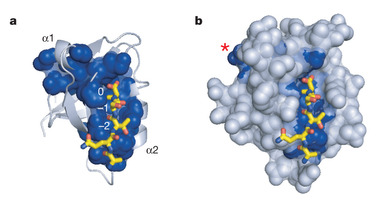
\includegraphics[width=10cm]{Images/pdz.jpg}
	\caption{\textbf{Left}: We show the PDZ domain (in blue) with the target peptide (yellow). The C-terminal of the target peptide is numbered 0 whilst the preceding amino acids are numbered in descending order. 
	\textbf{Right}: The position of the PDZ-Domain within the parent protein is shown. The position marked with a little star shows that during the binding process there are other parts of the PDZ domain which are involved and not just the binding pocket}
	\end{figure}	

	\section{Explanation of the data of Stifler et al}

	Now that we have given a small introduction to PDZ domains we shall explain the work done by Stifler and co-authors which we sought to extend and improve upon.

	The article that we have considered is titled "PDZ domain binding specificity is optimized across the mouse proteome". In this article, Michael Stifler and co-authors sought to characterize the selectivity between 157 PDZ domains and 217 target peptides found in the mouse proteome. To this end, they created a model which could predict whether a given PDZ domain would bind to a target peptide given the sequence of the target peptide.

	In their model, the last 5 positions near the C-terminal of the target peptide are considered. The model can be summarized in the following simple equation: 

	\begin{align}
	\label{model_base}
	\phi_{i} = \sum_{p,q} A_{p,q} \theta_{i,p,q} > \tau_{i}
	\end{align}

	where for a given PDZ Domain $i$, we can calculate a binding score $\phi_{i}$. $A$ is an indicator of the peptide sequence : $A_{p,q} =1$ if the amino acid at position $p$ of the peptide is $q$ and $A_{p,q} =0$ otherwise. The numbers $\theta_{i,p,q}$ are the parameters that need to be fit to the experimental data. $\tau_{i}$ is a scoring threshold which is different for each domain $i$. The values $\theta_{i,p,q}$ are to be interpreted in the following fashion: $\theta_{i,p,q} > 0$ if the PDZ Domain $i$ prefers amino acid $q$ at position $p$ more than the other PDZ domains, negative if it prefers it less, and 0 if it has no bias relative to the other domains. $\tau_{i}$ is defined as the $m$th percentile of the $\phi_{i}$'s for all the peptides in the model that bound to the domain $i$. To make predictions using this model, it suffices to know the sequence of the target peptide and compute $\phi_{i} - \tau_{i}$ for the domain $i$. If the domain binds with the target protein then this number is positive and negative otherwise. 

	The data used to fit the model was obtained by protein micro-array assays. Each PDZ Domain-peptide pair under consideration was verified for binding during the experiment. The researchers were able to model 74 domains among the 157 domains experimented upon. The experimental results of these experiments are available to us in the form of an interaction matrix which tells us whether a PDZ domain $i$ binds to a target peptide $j$ or not. 

	For each of the 74 domains successfully modeled, we also possess the parameters $\theta_{i,p,q}$ allowing us to test the model on newer peptide sequences. We also possess the error rates for the model. These are given in terms of false positive and false negative rates. These error rates interpreted as empirical probabilities were used in one of the models presented later in the report.

	\section{Questions asked and answered}

	With the biological context established and the various data that we possess explained, let us now briefly the discuss the questions that we sought to answer over the course of the project. 

	Firstly, we sought to understand the effect of mutations on the specificity of domain-peptide interactions. It is well known that PDZ domains bind to only certain specific target peptides and not to others. What if the target peptide suffered a point mutation? Will the PDZ domain still bind to the peptide? 

	A related question concerns the level of constraint imposed on the peptides due to the specificity of their interactions with PDZ domains. If the peptide were to suffer a point mutation and if it continued to bind to the PDZ domain, it then becomes interesting to consider the extent to which the peptide can undergo mutations before it stops binding to the peptide. Inversely, if the peptide doesn't accept many mutations, it is again interesting to analyze whether there are certain positions or amino acids which impose constraints on the sequence. 

	All such questions were modeled, analyzed and understood in this project.

\pagebreak
\part{First Model}
	\section{Features of the model}

	Our first model sought to study the effects of the introduction of mutations in the target peptide sequences conserving all the while the interaction matrix. The mutations considered were point mutations whereby one amino acid at a particular position was muted into another one. To this end, we define a parameter $\alpha$ which corresponds to binding or non-binding for the domain-peptide pair in the interaction matrix, $\alpha=1$ if PDZ domain $i$ binds to peptide $j$ and $\alpha = -1$ otherwise. Since we want to introduce mutations that conserve the interaction matrix, we begin with the natural sequence of a given peptide and introduce mutations in the natural sequence. 

	Now, we start from a natural sequence of the peptide $l$. Once a point mutation has been introduced in the sequence, we calculate the binding score $\phi$ for this new sequence using \eqref{model_base}. We then define a probability of binding and non-binding in the following manner:

	\begin{align}
	\label{model_1_naive}
	p(\alpha_{i,l}=1) & = \frac{1}{1+e^{-\phi}} \\
	p(\alpha_{i,l}=-1) & = \frac{1}{1+e^{\phi}}
	\end{align}

	for the domain $i$ and peptide $l$. Here we continue to use the label $l$ for the peptide even though the \emph{new} binding score $\phi$ is calculated for a mutated sequence and not the natural sequence for the peptide $l$

	Furthermore, we define an \emph{energy} for each peptide $l$ as:

	\begin{equation}
	\label{model_1_energy}
	\mathrm{E} = \sum_{i} \mathrm{log}(1+e^{-\alpha_{i,l}\phi_{i,l}})
	\end{equation}

	where the sum is over all domains $i$ in our data set. The energy defined can thus be defined for any sequence derived by introducing point mutations into the base sequence of the peptide $l$. In practice, we have a natural sequence, we then introduce a mutation into the sequence, calculate the probabilities $p(\alpha=1)$ or $p(\alpha=-1)$ for a given domain $i$ and sum the natural logs of these probabilities over all the 74 domains. 

	Once the mutations have been introduced and an energy defined for a new sequence derived from some natural peptide sequence, we now need a method to determine whether we accept or reject these mutations. To this end, we adopt the Metropolis algorithm, used for performing Monte Carlo simulations. The choice of performing a Monte Carlo simulation is a natural one since the sequence space consists of $20^5$ sequences and rather than sampling the whole space uniformly, it is more economical to perform a Monte Carlo (hereby MC) simulation.

	The general flow of the simulations was as follows:

	\begin{enumerate}
	\item 
	We begin with a single peptide and introduce point mutations starting with the natural sequence of the peptide. 
	\item 
	We then compare the energies, as defined in \eqref{model_1_energy}, between two sequences $\mathrm{E}_{old}$ and $\mathrm{E}_{new}$. 
	\item 
	We then use the Boltzmann factor to attribute probabilities to each of the energies  $\mathrm{E}_{old}$ and $\mathrm{E}_{new}$, where the boltzmann factor is 
	\begin{align}
	\label{boltz}
	p(E) \propto e^{-\beta E}
	\end{align}

	where $\beta$ is called the inverse temperature and the factor of proportionality is the partition function. Since we will take ratios of probabilities, we need not compute the partition function explicitly. 

	\item 
	We define the acceptance probability as :

	\begin{align}
	\label{prob_acceptance}
	p_{\mathrm{accept}} = \mathrm(min(1, \frac{p_{new}}{p_{old}}))
	\end{align}

	where $p_{new}$ and $p_{old}$ are computed using the Boltzmann factor.

	\item 

	Given $u \in U[0,1]$ where $U[0,1]$ is the uniform probability distribution, the new sequence is accepted if $ u < p_{\mathrm{accept}}$
	\end{enumerate}

	We chose the value of $\beta=1$. We performed 10 cycles of Monte Carlo runs, whereby during each run we affected 1000 mutations to each of the 217 peptides in our data set. 

 	\section{Results}

 	The first quantity that we computed was the initial distribution of energies i.e. energies computed for each of the peptides using only their natural sequences. 

 	\begin{figure}
 	\label{hist_ini_energies}
 	\centering
 	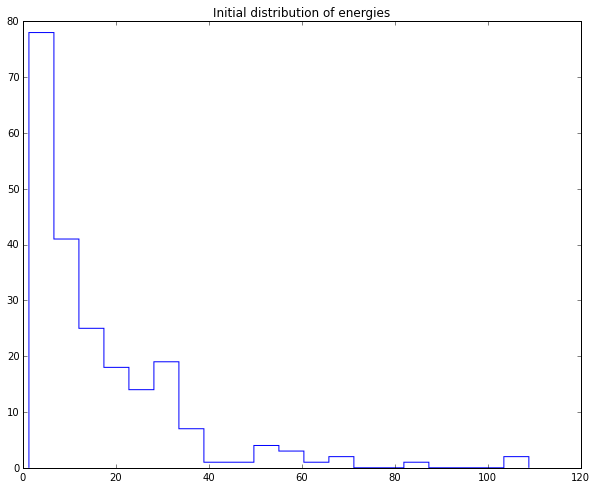
\includegraphics[width=8cm]{Images/hist_ini_energies.png}
 	\caption{The distribution of initial energies of the peptides. We observe that the energies are well spread out, with the majority in the range from 0-5 and the maximum energy close to 100}
 	\end{figure}

 	We compare this distribution to the distribution of energies of those sequences which were accepted during the Monte Carlo runs

 	\begin{figure}[!h]
 	\label{hist_final_energies} 
 	\centering
 	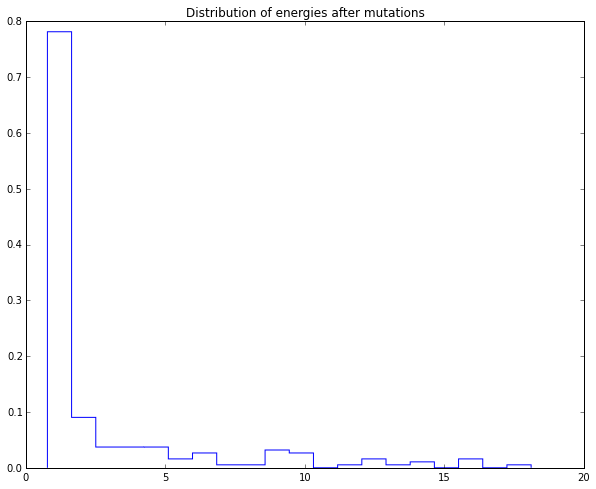
\includegraphics[width=8cm]{Images/hist_fin_energies.png}
 	\caption{Here the spread is reduced. The maximum is close to 19.}
 	\end{figure} 

 	We see a reduction by a factor of 5 in the spread of energies before and after the Monte Carlo runs.

 	The next quantity that we considered was the probability of having a given amino acid at any position for any peptide. To this end, we computed the frequency matrix which tells us how often a given amino acid was accepted during the Monte Carlo runs. 

 	\begin{figure}[!h]
 	\label{freq_matrix}
 	\centering
 	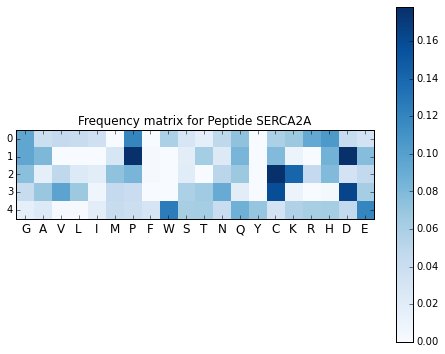
\includegraphics[width=7cm]{Images/freq_matrix.png}
 	\caption{The frequency matrix gives a very simple and visual way of deciding whether a given peptide is susceptible of undergoing mutations.} 
 	\end{figure}

 	Here the peptide considered \textbf{SERCA2A} has the sequence \textbf{PAILE}. We observe that the most frequent amino acid during the MC runs was Proline(P) and not Alanine (A). Thus we can already see that this peptide is susceptible to undergo mutations. This claim is further supported with the spread over all the 20 amino acids. 

 	The peptide \textbf{Cftr} presents a rather particular case for us. Its frequency matrix is presented here. We remark very clearly how, except for the last position, the other positions are not susceptible at all to undergo mutations. Even the mutations that do occur in the last position are not drastic. The natural sequence of \textbf{Cftr} is \textbf{QETRL}. On the last position, we see that the only mutation accepted is a transformation from Leucine (L) to Isoleucine, which would not be sterically important. Thus we find an interesting case of the existence of strong constraints on the sequence of the peptides in the face of mutations. During the MC runs, \textbf{Cftr} oscillates between two sequences: natural sequence \textbf{QETRL} and a mutated sequence \textbf{QETRI} 

 	\begin{figure}
 	\label{cft_freq}
 	\centering
 	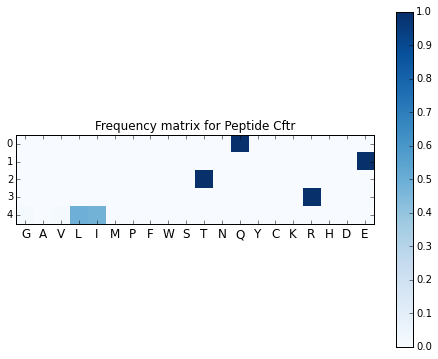
\includegraphics[width = 7cm]{Images/cftr.png}
 	\caption{The sequence for \textbf{Cftr} is very strictly constrained accepting mutations only at the last position.}
 	\end{figure} 

 	\section{Limitations}

 	This model however is not without its limitations. Another particular case that we consider is the peptide \textbf{APC} which has the natural sequence \textbf{LVTSV} and has a natural energy of 108. When we consider the evolution of the energy over the course of any one MC cycle, we observe that it has a tendency to very quickly reduce its energy as is evident from the plot below

 	\begin{figure}[!h]
 	\label{apc_evol}
 	\centering
 	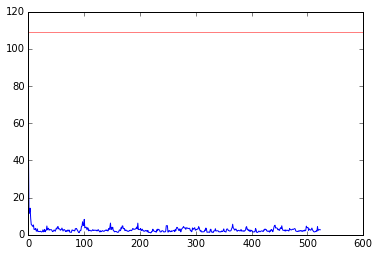
\includegraphics[width=7cm]{Images/apc_evol.png} 
 	\caption{The evolution of the energies of the mutated sequences of \textbf{APC} during one MC cycle. Out of 1000 mutations possible, it accepts close to 530 mutations, showing a great susceptibility to undergo mutations. Red line show the natural energy.}
 	\end{figure} 

 	This behavior is related to the particular nature of the peptide \textbf{APC} as well as the errors inherent in the model. We ascribe this behavior to the erroneous predictions of the model which needs to be accounted for in a newer model. This is the subject of the next section. 
\part{Improvements over first model: Bayesian Modeling}
	\section{Error rates as probabilities}
	\section{Updated Bayesian model}
	\section{Improvements over first model}
	\section{Results}
	\section{Interesting observations}
\part{Integrating PDZ Domain sequences} 
	\section{The LASSO}
	\section{Interesting observations}
\part{Conclusion}

\end{document}